\documentclass[aspectratio=169,t,xcolor=table]{beamer}
\usepackage[utf8]{inputenc}

\usepackage{booktabs} 
\usepackage{subcaption}
\usepackage{epigraph}
\usepackage[outercaption]{sidecap}    
\usepackage{tikz}


\usetheme{Ufg}

%-------------------------------------theorems--------------
\newtheorem{conj}{Conjetura}
\newtheorem{defi}{Definition}
\newtheorem{teo}{Teorema}
\newtheorem{lema}{Lema}
\newtheorem{prop}{Proposição}
\newtheorem{cor}{Corolário}
\newtheorem{ex}{Example}
\newtheorem{exer}{Exercício}

\setbeamertemplate{theorems}[numbered]
\setbeamertemplate{caption}[numbered]

%-------------------------------------------------------------%
%----------------------- Primary Definitions -----------------%

\definecolor{color1}{RGB}{0,0,90} % Color of the article title and sections
\definecolor{color2}{RGB}{0,20,20} % Color of the boxes behind the abstract and headings
\definecolor{keys1}{rgb}{0.0, 0.29, 0.33}
\definecolor{keys2}{rgb}{0.25, 0.7, 0.55}
\definecolor{keys3}{rgb}{0.1, 0.3, 0.4}
\definecolor{keys4}{rgb}{0.21, 0.46, 0.53}
\definecolor{strings}{rgb}{0.0, 0.47, 0.44}
\definecolor{comments}{rgb}{0.4, 0.4, 0.5}
\definecolor{terminaltext}{rgb}{1,1,1}
\definecolor{terminalbackground}{rgb}{0.2,0.2,0.25}

\usepackage{listings}

\usepackage{hyperref}
\hypersetup{
    colorlinks=true,
    linkcolor=blue,
    filecolor=magenta,      
    urlcolor=red,
    pdftitle={Overleaf Example},
    pdfpagemode=FullScreen,
    }

\lstset{
  xleftmargin=8pt,
  xrightmargin=0pt,
  framexleftmargin=0pt,
  framexrightmargin=0pt,
  basicstyle={\fontsize{8pt}{10pt}\ttfamily},
  columns=flexible,
  keepspaces=false,
  showstringspaces=false,
  commentstyle= \color{comments},
  stringstyle= \color{strings},
  breaklines=false,
  postbreak=\mbox{$\hookrightarrow$\space}
}

\lstdefinelanguage{Terminal}{
  framexleftmargin=3pt,
  framexrightmargin=3pt,
  framextopmargin=3pt,
  framexbottommargin=3pt,
  backgroundcolor=\color{terminalbackground},
  basicstyle={\fontsize{8pt}{10pt}\ttfamily\color{terminaltext}},
}

%%% Bibliography
\usepackage[style=numeric,backend=biber]{biblatex}
\addbibresource{thud.bib}


% This command set the default Color, is also possible to choose a custom color
\setPrimaryColor{UFGBlue} 

% First one is logo in title slide (we recommend use a horizontal image), and second one is the logo used in the remaining slides (we recommend use a square image)
\setLogos{lib/logos/infw.png}{lib/logos/infw2.png} 

% -------------------------------------- Title Slide Information
\begin{document}
\title[Inf UFG]{AI for State Estimation}
\subtitle{Project}

\author{Zanolin Lorenzo\inst{1}}

\institute[UFG] % (optional)
{
  \inst{1}%
  Control of Networked Systems\\
  Universität Klagenfurt
}
\date{February 2024}
%-----------------------The next statement creates the title page.
\frame[noframenumbering]{\titlepage}

%------------------------------------------------Slide 1
\setLayout{vertical} % This command define the layout. 'vertical' can be replace with 'horizontal', 'blank, 'mainpoint', 'titlepage'

\begin{frame}
    \frametitle{Table of Contents}
    \tableofcontents
\end{frame}
%---------------------------------------------------------

\section{Introduction}

\setLayout{mainpoint}
\setBGColor{DarkPurple}
\begin{frame}{}
    \frametitle{Introduction}
\end{frame}
\setLayout{vertical}

\begin{frame}
    \frametitle{Project description}
    The aim of the project is to use AI for state estimation; in this case we will implement some NN architectures to predict changes in heading angle and displacement using as data IMU data recorded using ROS gazebo simulator.\\
    \vspace{5mm}
    We will use TurtleBot3 as mobile robot to get the measurements inside the Gazebo environment; for convenience, we created the python script \textit{turtlebot3\_waypoints.py} to record the bagfiles from the simulations.\\
    \vspace{5mm} 

In this script we will save the output as bagfile, then it will be indexed to reduce the its size; finally we will pass as input to the NN 10 runs as training data and then the network will be evaluated on a new run to predict the waypoints.
\end{frame}

\begin{frame}[allowframebreaks]{Steps}
    To summarize, we will do the following steps:
    \begin{enumerate}
        \item Launch TurtleBot3 inside Gazebo.
        \begin{block}

            cd \textasciitilde/catkin\_ws\\
            catkin\_make\\
            source devel/setup.bash\\
            export TURTLEBOT3\_MODEL=burger\\
            roslaunch turtlebot3\_gazebo turtlebot3\_world.launch
        \end{block} 
        \item Run the Navigation node to do Initial Pose estimation and to collect some of the surrounding environment information.
        \begin{block}
            
            export TURTLEBOT3\_MODEL=burger\\
            roslaunch turtlebot3\_navigation turtlebot3\_navigation.launch \\ 
            \quad map\_file:=\$HOME/map.yaml
        \end{block} 
        \item Launch the script \textit{turtlebot3\_waypoints.py} to record the bagfile from the simulation.
        \begin{block}
            
            roslaunch turtlebot3\_waypoints turtlebot3\_waypoints.launch\\
            \quad bagfile:=/home/lorenzo/runs/run.bag
        \end{block} 
        In our case we will use 11 different waypoints arrays, thus we will end with 10 runs (which will be used as training data) and a test run.
        \item Index all the obtained bagfiles to reduce the size of them.
        \begin{block}
            
            rosbag reindex run.bag
        \end{block} 
        \item Launch the NN with the obtained run and record the results.
    \end{enumerate}
    Now, we will briefly report the used NN architectures and the hyperparameters; we have used LSTM and Transformer as general structure.
\end{frame}

\section{Architectures}

\setLayout{mainpoint}
\setBGColor{Ocean}
\begin{frame}{}
    \frametitle{Architectures}
\end{frame}
\setLayout{vertical}

\begin{frame}{Some details}
    %riassumi le architetture con le caratteristiche
    %riassumi tutte le combinazioni di hyperp
    The used architectures are:
    \begin{itemize}
        \item LSTM \cite{yu2019review}
        \item Transformer \cite{vaswani2017attention}
    \end{itemize}
    As for the parameters:
    \begin{itemize}
        \item Adam as optimizer (also with weight decay $wd=0.01$)
        \item learning rate $lr \in \{0.0002,0.0001,0.0005,0.001\}$.
        \item step size $step\_size \in \{50,100,200,300\}$.
        \item gamma $gamma \in \{0.01,0.1,0.2\}$.
        \item number of epochs $epochs \in \{10,15,20,25,50,100\}$.
        \item batch size $batch \in \{16,32,64,128\}$.
        \item hidden size $hidden \in \{6,64,128,256\}$.
    \end{itemize}  
\end{frame}

\section{Measurements}

\setLayout{mainpoint}
\setBGColor{LightOrange}
\begin{frame}{}
    \frametitle{Measurements}
\end{frame}
\setLayout{vertical}

\begin{frame}[allowframebreaks]{Experiment}
We will briefly report a short table demonstrating the best results for each architecture; the complete results table can be found in my \href{https://github.com/lorenzozanolin/StateEstimation}{GitHub repo}.%link github.
\begin{table}[]
    \begin{tabular}{|c|c|c|c|c|c|c|c|c|}
    \hline
    \textbf{model} & \textbf{epochs} & \textbf{batch size} & \textbf{train loss} & \textbf{test loss} \\ \hline
    LSTM                                  & 20                                     & 32                                         & 0.1668              & 0.3618             \\ \hline
    Transformer, dropout = 0.7            & 10                                     & 64                                         & 0.3181               & 0.3780             \\ \hline
    \end{tabular}
    \end{table}
As we can see, we obtained slightly better results using LSTMs; the runs were done mainly on CPU, thus the required time per epoch was always around 2-3 minutes for bigger batch sizes, while for the smaller ones (4-8) the model required almost 20 minutes per epoch.\\
\vspace{5mm}
We will now show the obtained graphs of the errors w.r.t. the number of epochs.\\
\vspace{4mm}
Results with LSTM:
\begin{figure}[!htb]
    \begin{center}
        \begin{minipage}{0.45\textwidth}
            \centering
            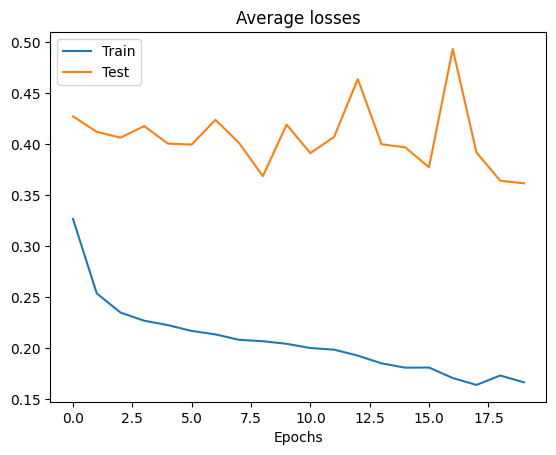
\includegraphics[width=\linewidth]{../outputs/lstmError.png}
            \caption{Errors}\label{graph1}
        \end{minipage}
        \hfill
        \begin{minipage}{0.45\textwidth}
            \centering
            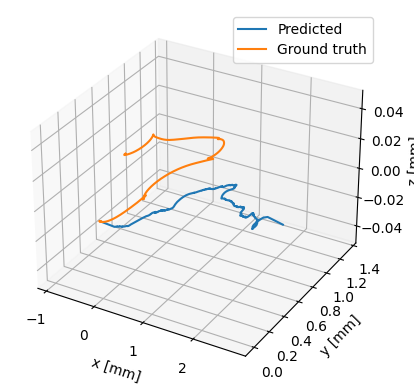
\includegraphics[width=\linewidth]{../outputs/lstmTrajectory.png}
            \caption{Estimated trajectory.}\label{graph2}
        \end{minipage}
    \end{center}
\end{figure}
Results with Transformer:
\begin{figure}[!htb]
    \begin{center}
        \begin{minipage}{0.45\textwidth}
            \centering
            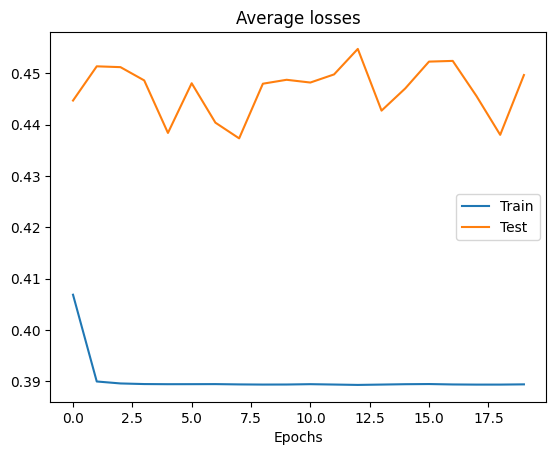
\includegraphics[width=\linewidth]{../outputs/transformerError.png}
            \caption{Errors}\label{graph3}
        \end{minipage}
        \hfill
        \begin{minipage}{0.45\textwidth}
            \centering
            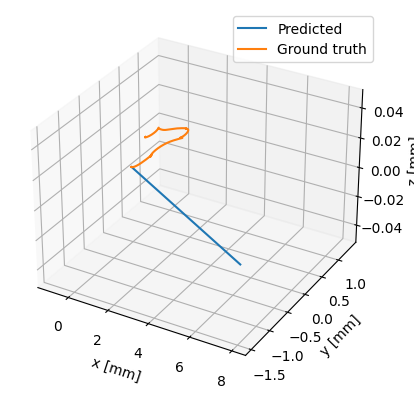
\includegraphics[width=\linewidth]{../outputs/transformerTrajectory.png}
            \caption{Estimated trajectory.}\label{graph4}
        \end{minipage}
    \end{center}
\end{figure}

As observed, the train error of the LSTM appears to decrease steadily with each epoch, whereas for the Transformer, it seems to stabilize around $0.3$. \\
\vspace{5mm}

However, for the test error, both models exhibit fluctuations across different values.\\
\vspace{5mm}
Note: All LSTM measurements were done using Colab standard CPU (Intel Xeon CPU with 2 vCPUs and 13GB of RAM), while Transformer ones were done on a M1 Pro 10 core.\\
\end{frame}

\section{Conclusions}

\setLayout{mainpoint}
\setBGColor{LightGray}
\begin{frame}{}
    \frametitle{Conclusions}
\end{frame}
\setLayout{vertical}

\begin{frame}{To conclude}
    In conclusion, while the experiments testing state estimation using LSTM and Transformers resulted in suboptimal results, the process proved invaluable in gaining a deeper understanding of their functionality.\\ \vspace{5mm} We did various adjustments of hyperparameters and architectures (switching between the two), thus we have enhanced our comprehension of their capabilities and structure.
\end{frame}

\begin{frame}[allowframebreaks]{References}
    \nocite{*} 
    \printbibliography
\end{frame}

\end{document}